\chapter{Bayesian neural network surrogate}
\section{Bayesian Neural Networks}
Bohamiann and numpyro-BNN are examples of probabilistic models with intractable inference. The predictive density is given as, 
\begin{align*}
    p(y_*|x_*,\mathcal{D}) &= \int p(y_*|x, \theta)p(\theta|\mathcal{D})d\theta\\
    &\approx \frac{1}{K} \sum_{k=1}^K p(y_*|x, \theta^{(k)})
\end{align*}
where the first integral is intractable as $\theta$ can live in a highly dimensional space, second the approximation sign
is true, since we can aproximate the integral with monte carlo sampling: $\theta^{(k)}$ are iid samples from the posterior 
distribution, $\theta^{(k)} \sim p(\theta|\mathcal{D})$. We can get samples from the posterior distriution

\begin{testexample2}[Monte Carlo approximation]
    Assuming we have a number of iid samples, $\theta^{(1)}, \dots, \theta^{(K)}$ drawn from the
    distribution $p(x)$, then the following appriximation 
    $$E[f(x)] \approx \frac{1}{K} \sum_{k=1}^K f(x^{(k)}) =: \Theta_{K}(f)$$
    holds accoring to the law of large numbers 
    in fact $$E[f(x)] = \lim_{K \rightarrow \infty} \Theta_{K}(f)$$
    and the central limit theorem, <OBS refere!>
    $$p(\hat \Theta) \approx \mathcal{N}(\hat \Theta |\mu_f, \frac{\sigma_f^2}{K})$$
    which ensures that the variance of the unbiased estimator of the expecation decreases
    with number of samples, $K$. Left is to sample the $iid$ samples from the distribution $p(x)$
\end{testexample2}
\subsection*{Posterior samples}
For both models 
the joint distribution $p(\mathcal{D},\theta)$ is available, but calulating the posterior distribution requires the
marginalized likehood, $p(\mathcal{D}) = \int_{\theta} p(\mathcal{D},\theta)$. This integral is often intractable
since the space of $\theta$ typically is abnomous - so not even nummerical appriximations of the intergral is tractable.
From Bayes rule, we have the equality, 
$$p(\theta|\mathcal{D}) = \frac{p(\mathcal{D},\theta)}{p(\mathcal{D})} \propto p(\mathcal{D},\theta),$$
where the propotional sign is true, since $p(\theta|\mathcal{D})$ is a function of $\theta$. 
Knowing the $p(\mathcal{D},\theta)$ joint distribution thereby allow for using Markov chain Monte Carlo
for sampling from the posterior distribution.  

\begin{testexample2}[Markov chain Monte Carlo]
    We can conviniently use MCMC for sampling from a probability density $p(x)$, with only the knowledge of a 
    propotional/unnormalised density $\hat p(x) \geq 0$ i.e
    $$\hat p(x) = c\cdot p(x) \hspace{1cm} c = \int \hat p(x) dx,$$
    where $\int \hat p(x) dx$ is a possible intractable integral. 
    An ergodic Markov chain/process is constructed, such that its stationary distribution is exactly $p(x)$, but only
    with the knowledge of $\hat p(x)$. 
\end{testexample2}

\begin{testexample}[Metropolis-Hasting (MH)]
    The most simple MCMC method is the Metropolis-Hasting algorithm. At iteration
    $n$ we have a sample $x_n$,
    \begin{enumerate}
        \item Propose $\hat x$ from a proposal density $q(x_n,\cdot)$
        \item Compute accptance probability $$\alpha(x_n,\hat x) = \min \left(1, \frac{p(\hat x)}{p(x_n)} \frac{q(\hat x, x_n)}{q(x_n,\hat x)}\right)$$
        \item Set the next sample $$x_{n+1} = \begin{cases}
            \hat x &\text{with probability } \alpha(x_n, \hat x)\\
             x_n &\text{with probability } 1-\alpha(x_n, \hat x)
        \end{cases}$$
    \end{enumerate}
    note that $\alpha(x_n,\hat x)$ requires $p(x)$, but since the algorithm only
    requires the fraction $\frac{p(\hat x)}{p(x_n)} = \frac{p(\hat x)\cdot c}{p(x_n)\cdot c} = \frac{\hat p(\hat x)}{\hat p(x_n)}$
    we only need $\hat p$. 
    
    \textbf{Proof:} Assuming discrete states, the transition probability between the states are given as, 
    $$p(x\rightarrow y) = \begin{cases}
        q(x,y)\alpha(x,y) & \text{if } x\neq y\\
        q(x,x) + \sum_{z\neq x} q(x,z)(1-\alpha(x,z)) & \text{if } x=y
    \end{cases}$$
    Now, let us look at the so-called \textit{detailed balance} relation, i.e. that if we are sampling from the
    stationary density we stay there at the next state. Assume $x\neq y$, 
    \begin{align*}
        p(x)p(x\rightarrow y) &= p(x)q(x,y)\alpha(x,y)\\
        &=p(x)q(x,y) \min \left(1, \frac{p(\hat x)}{p(x_n)} \frac{q(\hat x, x_n)}{q(x_n,\hat x)}\right)\\
        &= \min(p(x)q(x,y), p(y)q(y,x))
    \end{align*}
    Observing that the right hand side yields symmetric result in $x$ and $y$, therefore we obtain, 
    $$p(x)p(x\rightarrow y) = p(y)p(y\rightarrow x)$$
    and summing over $x$ on both sides yields,
    \begin{align}
        \sum_x p(x)p(x\rightarrow y) &= p(y) \sum_x p(y\rightarrow x)\\
        \implies \hspace{0.5cm} p(y) &= \sum_x p(x)p(x\rightarrow y)
    \end{align}
    similar conclusion will be obtained for $x = y$, all in all this reveals that $p(x)$ is in fact invariant for the chain
     $\{x_1, \dots , x_n\}$ and thereby that MH is a MCMC algorithm. 
\end{testexample}

% Markov assumption -> history doesn't matter
% Monte Carlo -> Random simulation
% best methods, use gradients. 

% Simulared skate board in a state park. Physic simulation. 
% Often the simulation moves back and fouth and end up in the 
% same point - this is called a U-turn. 

% find global curvature from just knowing the local curvature. 
% Simulation is moving more in the area with high prob. mass. 

% Gradients: Automated differentiation. 

% We want to evaluate integrals of the fom $$E[f(x)] = \int f(x)p(x)dx$$ where $x \in \mathbb{R}^n$ is a
% random vector under the distribution $p(x)$. we are interested in problems where the form of $f(x)$ or $p(x)$
% makes the integral intractalbe. 

% \begin{testexample}[Bayesian neural network]
%     Choosing $f := \mathcal{N}(y;NN_w(x), \sigma)$ and looking at $\theta := (w,\sigma)$ as the random quantaty
%     under the posterior distribution $p(\theta|\mathcal{D})$ we indeed have case of a intractalbe expectation
% \end{testexample}



% Transition density kernel (transtion matrix for finite discrete spaces) $p(x^{(k)}|x^{(k-1)})$



% c) the convergence rate is independent on the
% dimensionality, l. The latter property is in contrast to methods based on the deterministic numerical
% integration, which, in general, have a rate of convergence that slows down as the dimensionality
% increases.

HM with random walk transition is very simple and it comes with some serious disadvantages:
slow convergence speed, might stay in the same region for a long time and produces highly correlated sampels. 
We can do better by replacing the random walk with gradient-guided movements and intepretate the probability
landscape as a physical system.


\begin{testexample}[HMC]
The golden standard in MCMC is the Hamilton monte carlo, which exploits arguments from classical mechanics
around the Hamiltonian equations. This method leads to more efficient sampling as the Hamiltonian intepretation allows the system
to take regions with high probability mass into acound - this is optained using gradient
of the probability landscape.  $\frac{-\partial E(x)}{\partial x} $
 
We define PDF
$$p(x) = \frac{1}{Z_E}\exp(-E(x)),$$

where $E(x)$ is interpretted as the systems potential energy. Now, an latent vector $q$ is introduced in order
to represent the momentum of the system, which gives us the kinetic energy of the system. 

$$K(q) = \frac{1}{2}\sum_{i=1}^l q_i^2$$

Giving the Hamilton function and its coresponing distribution

$$H(x,q)= E(x)+K(q)$$

and 
\begin{align}
    p(x,q) &= \frac{1}{Z_H} \exp(-H(x,q))\\
    &= \frac{1}{Z_E} \exp(-E(x))\frac{1}{Z_K} \exp(-K(x))\\
    &= p(x)p(q)
\end{align}

The desired distribution $p(x)$ is found as the marginal of $p(x,q)$

\end{testexample}

since some intuition is now established around Hamiltonian Monte Carlo, 
we look a bit on the two versions used in Numpyro-BNN and Bohamiann, 

\subsection{No U-Turn sampling}

othen the physical simulation in HMC goes forth and back the same path, and we risk getting bad samples.
No U-turn (NUTS) sampling avoid this. 

\subsection{Adaptive stochatic HMC}


\begin{figure}[H]
    \centering
    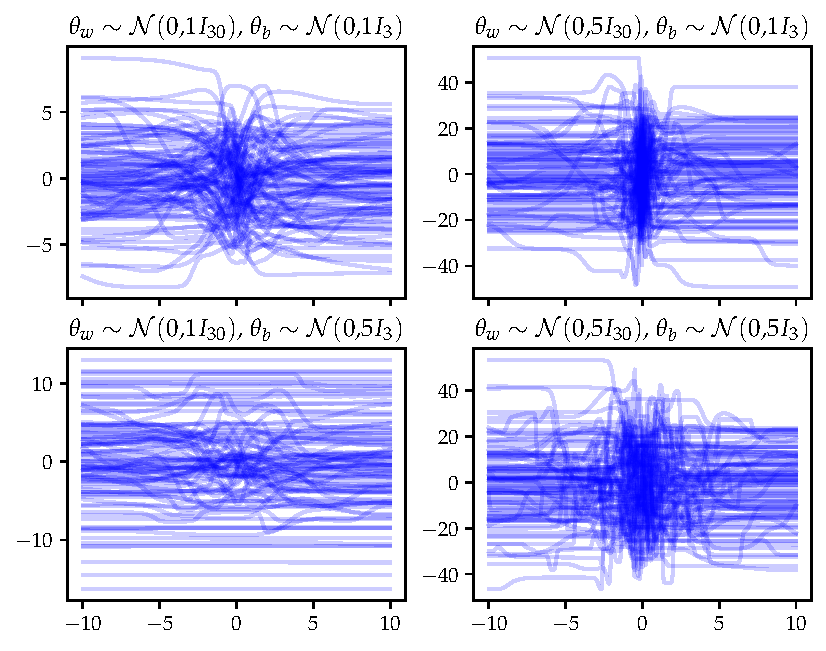
\includegraphics[width = \textwidth]{Pictures/bayesian_nn_prior_samples.pdf}
    \caption{Prior samples}
\end{figure}
\begin{figure}[H]
    \centering
    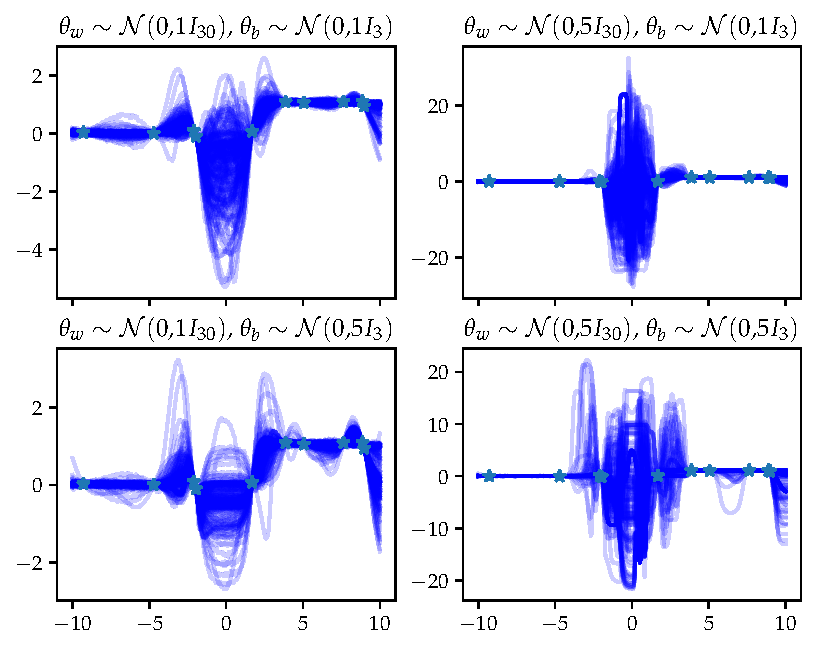
\includegraphics[width = \textwidth]{Pictures/bayesian_nn_posterior_samples.pdf}
    \caption{Posterior samples after observing }
\end{figure}